


\tikzset{every picture/.style={line width=0.75pt}} %set default line width to 0.75pt        

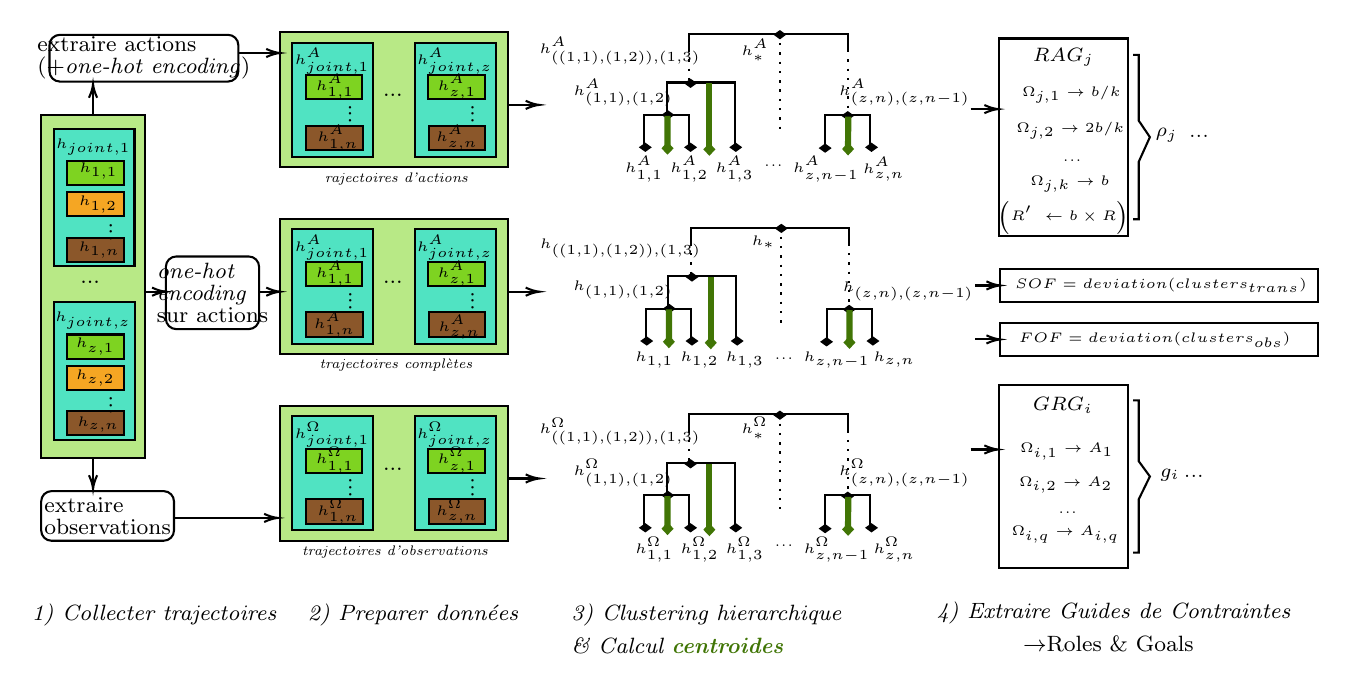
\begin{tikzpicture}[x=0.75pt,y=0.75pt,yscale=-1,xscale=1]
    %uncomment if require: \path (0,1974); %set diagram left start at 0, and has height of 1974

    %Shape: Rectangle [id:dp202038968054576] 
    \draw  [fill={rgb, 255:red, 184; green, 233; blue, 134 }  ,fill opacity=1 ] (45,1224) -- (95,1224) -- (95,1389) -- (45,1389) -- cycle ;
    %Shape: Rectangle [id:dp15280474832995194] 
    \draw  [fill={rgb, 255:red, 80; green, 227; blue, 194 }  ,fill opacity=1 ] (50.96,1230.4) -- (89.96,1230.4) -- (89.96,1296.76) -- (50.96,1296.76) -- cycle ;
    %Shape: Rectangle [id:dp01636589345867867] 
    \draw  [fill={rgb, 255:red, 245; green, 166; blue, 35 }  ,fill opacity=1 ] (57.44,1261.04) -- (84.69,1261.04) -- (84.69,1272.75) -- (57.44,1272.75) -- cycle ;
    %Shape: Rectangle [id:dp3662901515701339] 
    \draw  [fill={rgb, 255:red, 139; green, 87; blue, 42 }  ,fill opacity=1 ] (57.44,1282.91) -- (84.69,1282.91) -- (84.69,1294.62) -- (57.44,1294.62) -- cycle ;
    %Shape: Rectangle [id:dp2901229950076788] 
    \draw  [fill={rgb, 255:red, 126; green, 211; blue, 33 }  ,fill opacity=1 ] (57.44,1246.01) -- (84.69,1246.01) -- (84.69,1257.72) -- (57.44,1257.72) -- cycle ;
    %Shape: Rectangle [id:dp07258999584514214] 
    \draw  [fill={rgb, 255:red, 80; green, 227; blue, 194 }  ,fill opacity=1 ] (51,1314) -- (90,1314) -- (90,1380.37) -- (51,1380.37) -- cycle ;
    %Shape: Rectangle [id:dp8816488652434145] 
    \draw  [fill={rgb, 255:red, 245; green, 166; blue, 35 }  ,fill opacity=1 ] (57.48,1344.65) -- (84.72,1344.65) -- (84.72,1356.36) -- (57.48,1356.36) -- cycle ;
    %Shape: Rectangle [id:dp17661188452786847] 
    \draw  [fill={rgb, 255:red, 139; green, 87; blue, 42 }  ,fill opacity=1 ] (57.48,1366.51) -- (84.72,1366.51) -- (84.72,1378.22) -- (57.48,1378.22) -- cycle ;
    %Shape: Rectangle [id:dp7058774792564467] 
    \draw  [fill={rgb, 255:red, 126; green, 211; blue, 33 }  ,fill opacity=1 ] (57.48,1329.62) -- (84.72,1329.62) -- (84.72,1341.33) -- (57.48,1341.33) -- cycle ;
    %Shape: Rectangle [id:dp5049511033223727] 
    \draw  [fill={rgb, 255:red, 255; green, 255; blue, 255 }  ,fill opacity=1 ] (45,1410.08) .. controls (45,1407.32) and (47.24,1405.08) .. (50,1405.08) -- (104,1405.08) .. controls (106.76,1405.08) and (109,1407.32) .. (109,1410.08) -- (109,1424) .. controls (109,1426.76) and (106.76,1429) .. (104,1429) -- (50,1429) .. controls (47.24,1429) and (45,1426.76) .. (45,1424) -- cycle ;

    %Shape: Rectangle [id:dp7444540155367614] 
    \draw  [fill={rgb, 255:red, 184; green, 233; blue, 134 }  ,fill opacity=1 ] (160,1184) -- (270,1184) -- (270,1249) -- (160,1249) -- cycle ;
    %Shape: Rectangle [id:dp07209161659811003] 
    \draw  [fill={rgb, 255:red, 80; green, 227; blue, 194 }  ,fill opacity=1 ] (166,1189) -- (205,1189) -- (205,1244) -- (166,1244) -- cycle ;
    %Shape: Rectangle [id:dp16453391639267212] 
    \draw  [fill={rgb, 255:red, 139; green, 87; blue, 42 }  ,fill opacity=1 ] (172.76,1229) -- (200,1229) -- (200,1240.71) -- (172.76,1240.71) -- cycle ;
    %Shape: Rectangle [id:dp7339296953445047] 
    \draw  [fill={rgb, 255:red, 126; green, 211; blue, 33 }  ,fill opacity=1 ] (172.48,1204.62) -- (199.72,1204.62) -- (199.72,1216.33) -- (172.48,1216.33) -- cycle ;
    %Shape: Rectangle [id:dp9014627296605667] 
    \draw  [fill={rgb, 255:red, 80; green, 227; blue, 194 }  ,fill opacity=1 ] (225,1189) -- (264,1189) -- (264,1244) -- (225,1244) -- cycle ;
    %Shape: Rectangle [id:dp799025245782718] 
    \draw  [fill={rgb, 255:red, 139; green, 87; blue, 42 }  ,fill opacity=1 ] (231.76,1229) -- (259,1229) -- (259,1240.71) -- (231.76,1240.71) -- cycle ;
    %Shape: Rectangle [id:dp7036399386907127] 
    \draw  [fill={rgb, 255:red, 126; green, 211; blue, 33 }  ,fill opacity=1 ] (231.48,1204.62) -- (258.72,1204.62) -- (258.72,1216.33) -- (231.48,1216.33) -- cycle ;
    %Shape: Rectangle [id:dp9884197142173109] 
    \draw  [fill={rgb, 255:red, 184; green, 233; blue, 134 }  ,fill opacity=1 ] (160,1364) -- (270,1364) -- (270,1429) -- (160,1429) -- cycle ;
    %Shape: Rectangle [id:dp8777154281733445] 
    \draw  [fill={rgb, 255:red, 80; green, 227; blue, 194 }  ,fill opacity=1 ] (166,1369) -- (205,1369) -- (205,1424) -- (166,1424) -- cycle ;
    %Shape: Rectangle [id:dp7605476225941672] 
    \draw  [fill={rgb, 255:red, 139; green, 87; blue, 42 }  ,fill opacity=1 ] (172.76,1409) -- (200,1409) -- (200,1420.71) -- (172.76,1420.71) -- cycle ;
    %Shape: Rectangle [id:dp8039685412408772] 
    \draw  [fill={rgb, 255:red, 126; green, 211; blue, 33 }  ,fill opacity=1 ] (172.48,1384.62) -- (199.72,1384.62) -- (199.72,1396.33) -- (172.48,1396.33) -- cycle ;
    %Shape: Rectangle [id:dp02668095087444966] 
    \draw  [fill={rgb, 255:red, 80; green, 227; blue, 194 }  ,fill opacity=1 ] (225,1369) -- (264,1369) -- (264,1424) -- (225,1424) -- cycle ;
    %Shape: Rectangle [id:dp9793457024251365] 
    \draw  [fill={rgb, 255:red, 139; green, 87; blue, 42 }  ,fill opacity=1 ] (231.76,1409) -- (259,1409) -- (259,1420.71) -- (231.76,1420.71) -- cycle ;
    %Shape: Rectangle [id:dp7185879105671298] 
    \draw  [fill={rgb, 255:red, 126; green, 211; blue, 33 }  ,fill opacity=1 ] (231.48,1384.62) -- (258.72,1384.62) -- (258.72,1396.33) -- (231.48,1396.33) -- cycle ;
    %Straight Lines [id:da11923650827777166] 
    \draw    (140,1194) -- (158,1194) ;
    \draw [shift={(160,1194)}, rotate = 180] [color={rgb, 255:red, 0; green, 0; blue, 0 }  ][line width=0.75]    (6.56,-1.97) .. controls (4.17,-0.84) and (1.99,-0.18) .. (0,0) .. controls (1.99,0.18) and (4.17,0.84) .. (6.56,1.97)   ;
    %Shape: Rectangle [id:dp31005292076420676] 
    \draw  [fill={rgb, 255:red, 255; green, 255; blue, 255 }  ,fill opacity=1 ] (49,1190.24) .. controls (49,1187.48) and (51.24,1185.24) .. (54,1185.24) -- (135,1185.24) .. controls (137.76,1185.24) and (140,1187.48) .. (140,1190.24) -- (140,1202.76) .. controls (140,1205.52) and (137.76,1207.76) .. (135,1207.76) -- (54,1207.76) .. controls (51.24,1207.76) and (49,1205.52) .. (49,1202.76) -- cycle ;

    %Straight Lines [id:da33545170903821264] 
    \draw    (70,1224) -- (70,1211) ;
    \draw [shift={(70,1209)}, rotate = 90] [color={rgb, 255:red, 0; green, 0; blue, 0 }  ][line width=0.75]    (6.56,-1.97) .. controls (4.17,-0.84) and (1.99,-0.18) .. (0,0) .. controls (1.99,0.18) and (4.17,0.84) .. (6.56,1.97)   ;
    %Straight Lines [id:da34396155426267827] 
    \draw    (70,1389) -- (70,1402) ;
    \draw [shift={(70,1404)}, rotate = 270] [color={rgb, 255:red, 0; green, 0; blue, 0 }  ][line width=0.75]    (6.56,-1.97) .. controls (4.17,-0.84) and (1.99,-0.18) .. (0,0) .. controls (1.99,0.18) and (4.17,0.84) .. (6.56,1.97)   ;
    %Straight Lines [id:da38567178665573953] 
    \draw    (335.53,1422.76) -- (335.53,1407.15) -- (357.33,1407.15) -- (357.33,1422.76) ;
    %Straight Lines [id:da7572245576590513] 
    \draw    (346.43,1407.15) -- (346.43,1391.53) -- (379.12,1391.53) -- (379.12,1422.76) ;
    %Straight Lines [id:da3964198558123907] 
    \draw    (357.33,1375.91) -- (357.33,1368.11) -- (433.61,1368.11) -- (433.61,1375.91) ;
    %Straight Lines [id:da7473945747908602] 
    \draw    (422.71,1422.76) -- (422.71,1407.15) -- (444.51,1407.15) -- (444.51,1422.76) ;
    %Shape: Ellipse [id:dp40369424105740825] 
    \draw  [line width=2.25]  (335.53,1422.76) .. controls (335.53,1422.55) and (335.78,1422.37) .. (336.08,1422.37) .. controls (336.38,1422.37) and (336.62,1422.55) .. (336.62,1422.76) .. controls (336.62,1422.98) and (336.38,1423.15) .. (336.08,1423.15) .. controls (335.78,1423.15) and (335.53,1422.98) .. (335.53,1422.76) -- cycle ;
    %Shape: Ellipse [id:dp846189499167489] 
    \draw  [line width=2.25]  (357.33,1422.76) .. controls (357.33,1422.55) and (357.57,1422.37) .. (357.87,1422.37) .. controls (358.17,1422.37) and (358.42,1422.55) .. (358.42,1422.76) .. controls (358.42,1422.98) and (358.17,1423.15) .. (357.87,1423.15) .. controls (357.57,1423.15) and (357.33,1422.98) .. (357.33,1422.76) -- cycle ;
    %Shape: Ellipse [id:dp4518249986830597] 
    \draw  [line width=2.25]  (379.12,1422.76) .. controls (379.12,1422.55) and (379.37,1422.37) .. (379.67,1422.37) .. controls (379.97,1422.37) and (380.21,1422.55) .. (380.21,1422.76) .. controls (380.21,1422.98) and (379.97,1423.15) .. (379.67,1423.15) .. controls (379.37,1423.15) and (379.12,1422.98) .. (379.12,1422.76) -- cycle ;
    %Shape: Ellipse [id:dp7287955366321074] 
    \draw  [line width=2.25]  (422.17,1423.15) .. controls (422.17,1422.94) and (422.41,1422.76) .. (422.71,1422.76) .. controls (423.01,1422.76) and (423.26,1422.94) .. (423.26,1423.15) .. controls (423.26,1423.37) and (423.01,1423.54) .. (422.71,1423.54) .. controls (422.41,1423.54) and (422.17,1423.37) .. (422.17,1423.15) -- cycle ;
    %Shape: Ellipse [id:dp3895289499793816] 
    \draw  [line width=2.25]  (444.51,1422.76) .. controls (444.51,1422.55) and (444.75,1422.37) .. (445.05,1422.37) .. controls (445.35,1422.37) and (445.6,1422.55) .. (445.6,1422.76) .. controls (445.6,1422.98) and (445.35,1423.15) .. (445.05,1423.15) .. controls (444.75,1423.15) and (444.51,1422.98) .. (444.51,1422.76) -- cycle ;
    %Shape: Ellipse [id:dp8290194333831229] 
    \draw  [line width=2.25]  (346.43,1407.15) .. controls (346.43,1406.93) and (346.67,1406.75) .. (346.97,1406.75) .. controls (347.27,1406.75) and (347.52,1406.93) .. (347.52,1407.15) .. controls (347.52,1407.36) and (347.27,1407.54) .. (346.97,1407.54) .. controls (346.67,1407.54) and (346.43,1407.36) .. (346.43,1407.15) -- cycle ;
    %Shape: Ellipse [id:dp7432599113174565] 
    \draw  [line width=2.25]  (357.33,1391.92) .. controls (357.33,1391.7) and (357.57,1391.53) .. (357.87,1391.53) .. controls (358.17,1391.53) and (358.42,1391.7) .. (358.42,1391.92) .. controls (358.42,1392.14) and (358.17,1392.31) .. (357.87,1392.31) .. controls (357.57,1392.31) and (357.33,1392.14) .. (357.33,1391.92) -- cycle ;
    %Shape: Ellipse [id:dp7920805964261628] 
    \draw  [line width=2.25]  (400.37,1368.5) .. controls (400.37,1368.28) and (400.62,1368.11) .. (400.92,1368.11) .. controls (401.22,1368.11) and (401.46,1368.28) .. (401.46,1368.5) .. controls (401.46,1368.71) and (401.22,1368.89) .. (400.92,1368.89) .. controls (400.62,1368.89) and (400.37,1368.71) .. (400.37,1368.5) -- cycle ;
    %Shape: Ellipse [id:dp10334818761975828] 
    \draw  [line width=2.25]  (433.06,1407.54) .. controls (433.06,1407.32) and (433.31,1407.15) .. (433.61,1407.15) .. controls (433.91,1407.15) and (434.15,1407.32) .. (434.15,1407.54) .. controls (434.15,1407.75) and (433.91,1407.93) .. (433.61,1407.93) .. controls (433.31,1407.93) and (433.06,1407.75) .. (433.06,1407.54) -- cycle ;
    %Straight Lines [id:da7693959568996995] 
    \draw  [dash pattern={on 0.84pt off 2.51pt}]  (357.33,1375.91) -- (357.33,1391.53) ;
    %Straight Lines [id:da6041711886223101] 
    \draw  [dash pattern={on 0.84pt off 2.51pt}]  (433.61,1375.91) -- (433.61,1407.15) ;
    %Straight Lines [id:da5010636887023884] 
    \draw  [dash pattern={on 0.84pt off 2.51pt}]  (400.92,1368.11) -- (400.92,1414.95) ;
    %Straight Lines [id:da527245713439451] 
    \draw    (336.22,1332.76) -- (336.22,1317.15) -- (358.02,1317.15) -- (358.02,1332.76) ;
    %Straight Lines [id:da09936870625119643] 
    \draw    (347.12,1317.15) -- (347.12,1301.53) -- (379.81,1301.53) -- (379.81,1332.76) ;
    %Straight Lines [id:da696438929881343] 
    \draw    (358.02,1285.91) -- (358.02,1278.11) -- (434.3,1278.11) -- (434.3,1285.91) ;
    %Straight Lines [id:da26335679382262367] 
    \draw    (423.4,1332.76) -- (423.4,1317.15) -- (445.2,1317.15) -- (445.2,1332.76) ;
    %Shape: Ellipse [id:dp9550825383680106] 
    \draw  [line width=2.25]  (336.22,1332.76) .. controls (336.22,1332.55) and (336.47,1332.37) .. (336.77,1332.37) .. controls (337.07,1332.37) and (337.31,1332.55) .. (337.31,1332.76) .. controls (337.31,1332.98) and (337.07,1333.15) .. (336.77,1333.15) .. controls (336.47,1333.15) and (336.22,1332.98) .. (336.22,1332.76) -- cycle ;
    %Shape: Ellipse [id:dp9409194323440077] 
    \draw  [line width=2.25]  (358.02,1332.76) .. controls (358.02,1332.55) and (358.26,1332.37) .. (358.56,1332.37) .. controls (358.87,1332.37) and (359.11,1332.55) .. (359.11,1332.76) .. controls (359.11,1332.98) and (358.87,1333.15) .. (358.56,1333.15) .. controls (358.26,1333.15) and (358.02,1332.98) .. (358.02,1332.76) -- cycle ;
    %Shape: Ellipse [id:dp17984153815320425] 
    \draw  [line width=2.25]  (379.81,1332.76) .. controls (379.81,1332.55) and (380.06,1332.37) .. (380.36,1332.37) .. controls (380.66,1332.37) and (380.9,1332.55) .. (380.9,1332.76) .. controls (380.9,1332.98) and (380.66,1333.15) .. (380.36,1333.15) .. controls (380.06,1333.15) and (379.81,1332.98) .. (379.81,1332.76) -- cycle ;
    %Shape: Ellipse [id:dp4223131745323937] 
    \draw  [line width=2.25]  (422.86,1333.15) .. controls (422.86,1332.94) and (423.1,1332.76) .. (423.4,1332.76) .. controls (423.71,1332.76) and (423.95,1332.94) .. (423.95,1333.15) .. controls (423.95,1333.37) and (423.71,1333.54) .. (423.4,1333.54) .. controls (423.1,1333.54) and (422.86,1333.37) .. (422.86,1333.15) -- cycle ;
    %Shape: Ellipse [id:dp8557136991758003] 
    \draw  [line width=2.25]  (445.2,1332.76) .. controls (445.2,1332.55) and (445.44,1332.37) .. (445.74,1332.37) .. controls (446.05,1332.37) and (446.29,1332.55) .. (446.29,1332.76) .. controls (446.29,1332.98) and (446.05,1333.15) .. (445.74,1333.15) .. controls (445.44,1333.15) and (445.2,1332.98) .. (445.2,1332.76) -- cycle ;
    %Shape: Ellipse [id:dp7200174403259424] 
    \draw  [line width=2.25]  (347.12,1317.15) .. controls (347.12,1316.93) and (347.37,1316.75) .. (347.67,1316.75) .. controls (347.97,1316.75) and (348.21,1316.93) .. (348.21,1317.15) .. controls (348.21,1317.36) and (347.97,1317.54) .. (347.67,1317.54) .. controls (347.37,1317.54) and (347.12,1317.36) .. (347.12,1317.15) -- cycle ;
    %Shape: Ellipse [id:dp5512161172797779] 
    \draw  [line width=2.25]  (358.02,1301.92) .. controls (358.02,1301.7) and (358.26,1301.53) .. (358.56,1301.53) .. controls (358.87,1301.53) and (359.11,1301.7) .. (359.11,1301.92) .. controls (359.11,1302.14) and (358.87,1302.31) .. (358.56,1302.31) .. controls (358.26,1302.31) and (358.02,1302.14) .. (358.02,1301.92) -- cycle ;
    %Shape: Ellipse [id:dp9102331233634472] 
    \draw  [line width=2.25]  (401.06,1278.5) .. controls (401.06,1278.28) and (401.31,1278.11) .. (401.61,1278.11) .. controls (401.91,1278.11) and (402.15,1278.28) .. (402.15,1278.5) .. controls (402.15,1278.71) and (401.91,1278.89) .. (401.61,1278.89) .. controls (401.31,1278.89) and (401.06,1278.71) .. (401.06,1278.5) -- cycle ;
    %Shape: Ellipse [id:dp11911576725670614] 
    \draw  [line width=2.25]  (433.76,1317.54) .. controls (433.76,1317.32) and (434,1317.15) .. (434.3,1317.15) .. controls (434.6,1317.15) and (434.85,1317.32) .. (434.85,1317.54) .. controls (434.85,1317.75) and (434.6,1317.93) .. (434.3,1317.93) .. controls (434,1317.93) and (433.76,1317.75) .. (433.76,1317.54) -- cycle ;
    %Straight Lines [id:da5207212503133865] 
    \draw  [dash pattern={on 0.84pt off 2.51pt}]  (358.02,1285.91) -- (358.02,1301.53) ;
    %Straight Lines [id:da8576307598238995] 
    \draw  [dash pattern={on 0.84pt off 2.51pt}]  (434.3,1285.91) -- (434.3,1317.15) ;
    %Straight Lines [id:da16762679264131353] 
    \draw  [dash pattern={on 0.84pt off 2.51pt}]  (401.61,1278.11) -- (401.61,1324.95) ;
    %Straight Lines [id:da7226974109197233] 
    \draw    (335.53,1239.44) -- (335.53,1223.82) -- (357.33,1223.82) -- (357.33,1239.44) ;
    %Straight Lines [id:da7936026271252605] 
    \draw    (346.43,1223.82) -- (346.43,1208.21) -- (379.12,1208.21) -- (379.12,1239.44) ;
    %Straight Lines [id:da2016903467210477] 
    \draw    (357.33,1192.59) -- (357.33,1184.78) -- (433.61,1184.78) -- (433.61,1192.59) ;
    %Straight Lines [id:da4129095753823815] 
    \draw    (422.71,1239.44) -- (422.71,1223.82) -- (444.51,1223.82) -- (444.51,1239.44) ;
    %Shape: Ellipse [id:dp2665139577291352] 
    \draw  [line width=2.25]  (335.53,1239.44) .. controls (335.53,1239.22) and (335.78,1239.05) .. (336.08,1239.05) .. controls (336.38,1239.05) and (336.62,1239.22) .. (336.62,1239.44) .. controls (336.62,1239.66) and (336.38,1239.83) .. (336.08,1239.83) .. controls (335.78,1239.83) and (335.53,1239.66) .. (335.53,1239.44) -- cycle ;
    %Shape: Ellipse [id:dp031181712848845744] 
    \draw  [line width=2.25]  (357.33,1239.44) .. controls (357.33,1239.22) and (357.57,1239.05) .. (357.87,1239.05) .. controls (358.17,1239.05) and (358.42,1239.22) .. (358.42,1239.44) .. controls (358.42,1239.66) and (358.17,1239.83) .. (357.87,1239.83) .. controls (357.57,1239.83) and (357.33,1239.66) .. (357.33,1239.44) -- cycle ;
    %Shape: Ellipse [id:dp36682416413138486] 
    \draw  [line width=2.25]  (379.12,1239.44) .. controls (379.12,1239.22) and (379.37,1239.05) .. (379.67,1239.05) .. controls (379.97,1239.05) and (380.21,1239.22) .. (380.21,1239.44) .. controls (380.21,1239.66) and (379.97,1239.83) .. (379.67,1239.83) .. controls (379.37,1239.83) and (379.12,1239.66) .. (379.12,1239.44) -- cycle ;
    %Shape: Ellipse [id:dp21740668160132992] 
    \draw  [line width=2.25]  (422.17,1239.83) .. controls (422.17,1239.61) and (422.41,1239.44) .. (422.71,1239.44) .. controls (423.01,1239.44) and (423.26,1239.61) .. (423.26,1239.83) .. controls (423.26,1240.05) and (423.01,1240.22) .. (422.71,1240.22) .. controls (422.41,1240.22) and (422.17,1240.05) .. (422.17,1239.83) -- cycle ;
    %Shape: Ellipse [id:dp2823451915905191] 
    \draw  [line width=2.25]  (444.51,1239.44) .. controls (444.51,1239.22) and (444.75,1239.05) .. (445.05,1239.05) .. controls (445.35,1239.05) and (445.6,1239.22) .. (445.6,1239.44) .. controls (445.6,1239.66) and (445.35,1239.83) .. (445.05,1239.83) .. controls (444.75,1239.83) and (444.51,1239.66) .. (444.51,1239.44) -- cycle ;
    %Shape: Ellipse [id:dp10510163243452342] 
    \draw  [line width=2.25]  (346.43,1223.82) .. controls (346.43,1223.61) and (346.67,1223.43) .. (346.97,1223.43) .. controls (347.27,1223.43) and (347.52,1223.61) .. (347.52,1223.82) .. controls (347.52,1224.04) and (347.27,1224.21) .. (346.97,1224.21) .. controls (346.67,1224.21) and (346.43,1224.04) .. (346.43,1223.82) -- cycle ;
    %Shape: Ellipse [id:dp7198732993156373] 
    \draw  [line width=2.25]  (357.33,1208.6) .. controls (357.33,1208.38) and (357.57,1208.21) .. (357.87,1208.21) .. controls (358.17,1208.21) and (358.42,1208.38) .. (358.42,1208.6) .. controls (358.42,1208.81) and (358.17,1208.99) .. (357.87,1208.99) .. controls (357.57,1208.99) and (357.33,1208.81) .. (357.33,1208.6) -- cycle ;
    %Shape: Ellipse [id:dp2949740780410913] 
    \draw  [line width=2.25]  (400.37,1185.17) .. controls (400.37,1184.96) and (400.62,1184.78) .. (400.92,1184.78) .. controls (401.22,1184.78) and (401.46,1184.96) .. (401.46,1185.17) .. controls (401.46,1185.39) and (401.22,1185.57) .. (400.92,1185.57) .. controls (400.62,1185.57) and (400.37,1185.39) .. (400.37,1185.17) -- cycle ;
    %Shape: Ellipse [id:dp43678350565372726] 
    \draw  [line width=2.25]  (433.06,1224.21) .. controls (433.06,1224) and (433.31,1223.82) .. (433.61,1223.82) .. controls (433.91,1223.82) and (434.15,1224) .. (434.15,1224.21) .. controls (434.15,1224.43) and (433.91,1224.6) .. (433.61,1224.6) .. controls (433.31,1224.6) and (433.06,1224.43) .. (433.06,1224.21) -- cycle ;
    %Straight Lines [id:da31972831000851576] 
    \draw  [dash pattern={on 0.84pt off 2.51pt}]  (357.33,1192.59) -- (357.33,1208.21) ;
    %Straight Lines [id:da17231584437154546] 
    \draw  [dash pattern={on 0.84pt off 2.51pt}]  (433.61,1192.59) -- (433.61,1223.82) ;
    %Straight Lines [id:da590961207890984] 
    \draw  [dash pattern={on 0.84pt off 2.51pt}]  (400.92,1184.78) -- (400.92,1231.63) ;
    %Straight Lines [id:da4653804062230186] 
    \draw    (109,1418) -- (151.2,1418) -- (157,1418) ;
    \draw [shift={(159,1418)}, rotate = 180] [color={rgb, 255:red, 0; green, 0; blue, 0 }  ][line width=0.75]    (6.56,-1.97) .. controls (4.17,-0.84) and (1.99,-0.18) .. (0,0) .. controls (1.99,0.18) and (4.17,0.84) .. (6.56,1.97)   ;
    %Shape: Rectangle [id:dp7516919523559561] 
    \draw  [fill={rgb, 255:red, 184; green, 233; blue, 134 }  ,fill opacity=1 ] (160,1274) -- (270,1274) -- (270,1339) -- (160,1339) -- cycle ;
    %Shape: Rectangle [id:dp5758432318250756] 
    \draw  [fill={rgb, 255:red, 80; green, 227; blue, 194 }  ,fill opacity=1 ] (166,1279) -- (205,1279) -- (205,1334) -- (166,1334) -- cycle ;
    %Shape: Rectangle [id:dp16039269885325314] 
    \draw  [fill={rgb, 255:red, 139; green, 87; blue, 42 }  ,fill opacity=1 ] (172.76,1319) -- (200,1319) -- (200,1330.71) -- (172.76,1330.71) -- cycle ;
    %Shape: Rectangle [id:dp683608780334294] 
    \draw  [fill={rgb, 255:red, 126; green, 211; blue, 33 }  ,fill opacity=1 ] (172.48,1294.62) -- (199.72,1294.62) -- (199.72,1306.33) -- (172.48,1306.33) -- cycle ;
    %Shape: Rectangle [id:dp5938801905272854] 
    \draw  [fill={rgb, 255:red, 80; green, 227; blue, 194 }  ,fill opacity=1 ] (225,1279) -- (264,1279) -- (264,1334) -- (225,1334) -- cycle ;
    %Shape: Rectangle [id:dp7537224255422383] 
    \draw  [fill={rgb, 255:red, 139; green, 87; blue, 42 }  ,fill opacity=1 ] (231.76,1319) -- (259,1319) -- (259,1330.71) -- (231.76,1330.71) -- cycle ;
    %Shape: Rectangle [id:dp6800935225943223] 
    \draw  [fill={rgb, 255:red, 126; green, 211; blue, 33 }  ,fill opacity=1 ] (231.48,1294.62) -- (258.72,1294.62) -- (258.72,1306.33) -- (231.48,1306.33) -- cycle ;
    %Shape: Rectangle [id:dp22809977923512426] 
    \draw  [fill={rgb, 255:red, 255; green, 255; blue, 255 }  ,fill opacity=1 ] (105.08,1297.03) .. controls (105.08,1294.27) and (107.32,1292.03) .. (110.08,1292.03) -- (145,1292.03) .. controls (147.76,1292.03) and (150,1294.27) .. (150,1297.03) -- (150,1322.03) .. controls (150,1324.79) and (147.76,1327.03) .. (145,1327.03) -- (110.08,1327.03) .. controls (107.32,1327.03) and (105.08,1324.79) .. (105.08,1322.03) -- cycle ;

    %Straight Lines [id:da46588171274405754] 
    \draw    (95,1309) -- (103,1309) ;
    \draw [shift={(105,1309)}, rotate = 180] [color={rgb, 255:red, 0; green, 0; blue, 0 }  ][line width=0.75]    (6.56,-1.97) .. controls (4.17,-0.84) and (1.99,-0.18) .. (0,0) .. controls (1.99,0.18) and (4.17,0.84) .. (6.56,1.97)   ;
    %Straight Lines [id:da7862356264839616] 
    \draw    (150,1309) -- (158,1309) ;
    \draw [shift={(160,1309)}, rotate = 180] [color={rgb, 255:red, 0; green, 0; blue, 0 }  ][line width=0.75]    (6.56,-1.97) .. controls (4.17,-0.84) and (1.99,-0.18) .. (0,0) .. controls (1.99,0.18) and (4.17,0.84) .. (6.56,1.97)   ;
    %Straight Lines [id:da9867519450365554] 
    \draw    (270,1309) -- (283,1309) ;
    \draw [shift={(285,1309)}, rotate = 180] [color={rgb, 255:red, 0; green, 0; blue, 0 }  ][line width=0.75]    (6.56,-1.97) .. controls (4.17,-0.84) and (1.99,-0.18) .. (0,0) .. controls (1.99,0.18) and (4.17,0.84) .. (6.56,1.97)   ;
    %Straight Lines [id:da7183529744954437] 
    \draw    (270,1399) -- (283,1399) ;
    \draw [shift={(285,1399)}, rotate = 180] [color={rgb, 255:red, 0; green, 0; blue, 0 }  ][line width=0.75]    (6.56,-1.97) .. controls (4.17,-0.84) and (1.99,-0.18) .. (0,0) .. controls (1.99,0.18) and (4.17,0.84) .. (6.56,1.97)   ;
    %Straight Lines [id:da9034058657626025] 
    \draw    (270,1219) -- (283,1219) ;
    \draw [shift={(285,1219)}, rotate = 180] [color={rgb, 255:red, 0; green, 0; blue, 0 }  ][line width=0.75]    (6.56,-1.97) .. controls (4.17,-0.84) and (1.99,-0.18) .. (0,0) .. controls (1.99,0.18) and (4.17,0.84) .. (6.56,1.97)   ;
    %Straight Lines [id:da2319974209029203] 
    \draw [color={rgb, 255:red, 65; green, 117; blue, 5 }  ,draw opacity=1 ][line width=2.25]    (346.77,1424.09) -- (346.81,1407.54) ;
    %Shape: Ellipse [id:dp07813451072664179] 
    \draw  [color={rgb, 255:red, 65; green, 117; blue, 5 }  ,draw opacity=1 ][line width=2.25]  (345.92,1423.18) .. controls (345.92,1422.67) and (346.3,1422.26) .. (346.77,1422.26) .. controls (347.24,1422.26) and (347.63,1422.67) .. (347.63,1423.18) .. controls (347.63,1423.68) and (347.24,1424.09) .. (346.77,1424.09) .. controls (346.3,1424.09) and (345.92,1423.68) .. (345.92,1423.18) -- cycle ;
    %Straight Lines [id:da8006350861738639] 
    \draw [color={rgb, 255:red, 65; green, 117; blue, 5 }  ,draw opacity=1 ][line width=2.25]    (366.94,1422.76) -- (366.94,1391.93) ;
    %Shape: Ellipse [id:dp07333156941470187] 
    \draw  [color={rgb, 255:red, 65; green, 117; blue, 5 }  ,draw opacity=1 ][line width=2.25]  (366.08,1423.68) .. controls (366.08,1423.17) and (366.47,1422.76) .. (366.94,1422.76) .. controls (367.41,1422.76) and (367.79,1423.17) .. (367.79,1423.68) .. controls (367.79,1424.18) and (367.41,1424.59) .. (366.94,1424.59) .. controls (366.47,1424.59) and (366.08,1424.18) .. (366.08,1423.68) -- cycle ;
    %Straight Lines [id:da36579471993791146] 
    \draw [color={rgb, 255:red, 65; green, 117; blue, 5 }  ,draw opacity=1 ][line width=2.25]    (433.77,1424.43) -- (433.81,1407.87) ;
    %Shape: Ellipse [id:dp20331162001366287] 
    \draw  [color={rgb, 255:red, 65; green, 117; blue, 5 }  ,draw opacity=1 ][line width=2.25]  (432.92,1423.51) .. controls (432.92,1423) and (433.3,1422.59) .. (433.77,1422.59) .. controls (434.24,1422.59) and (434.63,1423) .. (434.63,1423.51) .. controls (434.63,1424.01) and (434.24,1424.43) .. (433.77,1424.43) .. controls (433.3,1424.43) and (432.92,1424.01) .. (432.92,1423.51) -- cycle ;
    %Straight Lines [id:da5105497739784041] 
    \draw [color={rgb, 255:red, 65; green, 117; blue, 5 }  ,draw opacity=1 ][line width=2.25]    (347.44,1334.05) -- (347.47,1317.49) ;
    %Shape: Ellipse [id:dp7589275189494679] 
    \draw  [color={rgb, 255:red, 65; green, 117; blue, 5 }  ,draw opacity=1 ][line width=2.25]  (346.58,1333.13) .. controls (346.58,1332.62) and (346.97,1332.21) .. (347.44,1332.21) .. controls (347.91,1332.21) and (348.29,1332.62) .. (348.29,1333.13) .. controls (348.29,1333.64) and (347.91,1334.05) .. (347.44,1334.05) .. controls (346.97,1334.05) and (346.58,1333.64) .. (346.58,1333.13) -- cycle ;
    %Straight Lines [id:da7466037272738116] 
    \draw [color={rgb, 255:red, 65; green, 117; blue, 5 }  ,draw opacity=1 ][line width=2.25]    (367.61,1332.71) -- (367.61,1301.88) ;
    %Shape: Ellipse [id:dp6857778816036284] 
    \draw  [color={rgb, 255:red, 65; green, 117; blue, 5 }  ,draw opacity=1 ][line width=2.25]  (366.75,1333.63) .. controls (366.75,1333.12) and (367.13,1332.71) .. (367.61,1332.71) .. controls (368.08,1332.71) and (368.46,1333.12) .. (368.46,1333.63) .. controls (368.46,1334.14) and (368.08,1334.55) .. (367.61,1334.55) .. controls (367.13,1334.55) and (366.75,1334.14) .. (366.75,1333.63) -- cycle ;
    %Straight Lines [id:da7347404569040029] 
    \draw [color={rgb, 255:red, 65; green, 117; blue, 5 }  ,draw opacity=1 ][line width=2.25]    (434.44,1334.38) -- (434.47,1317.82) ;
    %Shape: Ellipse [id:dp9712786577828096] 
    \draw  [color={rgb, 255:red, 65; green, 117; blue, 5 }  ,draw opacity=1 ][line width=2.25]  (433.58,1333.46) .. controls (433.58,1332.96) and (433.97,1332.55) .. (434.44,1332.55) .. controls (434.91,1332.55) and (435.29,1332.96) .. (435.29,1333.46) .. controls (435.29,1333.97) and (434.91,1334.38) .. (434.44,1334.38) .. controls (433.97,1334.38) and (433.58,1333.97) .. (433.58,1333.46) -- cycle ;
    %Straight Lines [id:da5804972425850201] 
    \draw [color={rgb, 255:red, 65; green, 117; blue, 5 }  ,draw opacity=1 ][line width=2.25]    (346.77,1240.83) -- (346.81,1224.28) ;
    %Shape: Ellipse [id:dp49350286387336273] 
    \draw  [color={rgb, 255:red, 65; green, 117; blue, 5 }  ,draw opacity=1 ][line width=2.25]  (345.92,1239.92) .. controls (345.92,1239.41) and (346.3,1239) .. (346.77,1239) .. controls (347.24,1239) and (347.63,1239.41) .. (347.63,1239.92) .. controls (347.63,1240.42) and (347.24,1240.83) .. (346.77,1240.83) .. controls (346.3,1240.83) and (345.92,1240.42) .. (345.92,1239.92) -- cycle ;
    %Straight Lines [id:da9672639506528268] 
    \draw [color={rgb, 255:red, 65; green, 117; blue, 5 }  ,draw opacity=1 ][line width=2.25]    (366.94,1239.5) -- (366.94,1208.67) ;
    %Shape: Ellipse [id:dp510572796447454] 
    \draw  [color={rgb, 255:red, 65; green, 117; blue, 5 }  ,draw opacity=1 ][line width=2.25]  (366.08,1240.42) .. controls (366.08,1239.91) and (366.47,1239.5) .. (366.94,1239.5) .. controls (367.41,1239.5) and (367.79,1239.91) .. (367.79,1240.42) .. controls (367.79,1240.92) and (367.41,1241.33) .. (366.94,1241.33) .. controls (366.47,1241.33) and (366.08,1240.92) .. (366.08,1240.42) -- cycle ;
    %Straight Lines [id:da41383136662371545] 
    \draw [color={rgb, 255:red, 65; green, 117; blue, 5 }  ,draw opacity=1 ][line width=2.25]    (433.77,1241.17) -- (433.81,1224.61) ;
    %Shape: Ellipse [id:dp3489136333049525] 
    \draw  [color={rgb, 255:red, 65; green, 117; blue, 5 }  ,draw opacity=1 ][line width=2.25]  (432.92,1240.25) .. controls (432.92,1239.74) and (433.3,1239.33) .. (433.77,1239.33) .. controls (434.24,1239.33) and (434.63,1239.74) .. (434.63,1240.25) .. controls (434.63,1240.76) and (434.24,1241.17) .. (433.77,1241.17) .. controls (433.3,1241.17) and (432.92,1240.76) .. (432.92,1240.25) -- cycle ;
    %Shape: Rectangle [id:dp6950547105184206] 
    \draw   (506.61,1354) -- (568.43,1354) -- (568.43,1442.03) -- (506.61,1442.03) -- cycle ;
    %Shape: Rectangle [id:dp6804770559805788] 
    \draw   (506.61,1187.03) -- (568.43,1187.03) -- (568.43,1282) -- (506.61,1282) -- cycle ;
    %Straight Lines [id:da8493809433087859] 
    \draw    (492.81,1385.03) -- (504,1385.03) ;
    \draw [shift={(506,1385.03)}, rotate = 180] [color={rgb, 255:red, 0; green, 0; blue, 0 }  ][line width=0.75]    (6.56,-1.97) .. controls (4.17,-0.84) and (1.99,-0.18) .. (0,0) .. controls (1.99,0.18) and (4.17,0.84) .. (6.56,1.97)   ;
    %Straight Lines [id:da0017946321588515612] 
    \draw    (492.81,1221.03) -- (504,1221.03) ;
    \draw [shift={(506,1221.03)}, rotate = 180] [color={rgb, 255:red, 0; green, 0; blue, 0 }  ][line width=0.75]    (6.56,-1.97) .. controls (4.17,-0.84) and (1.99,-0.18) .. (0,0) .. controls (1.99,0.18) and (4.17,0.84) .. (6.56,1.97)   ;
    %Straight Lines [id:da07100007457842461] 
    \draw    (571.12,1194.94) -- (573.81,1194.94) -- (573.81,1226.6) -- (579.18,1234.52) -- (573.81,1246.39) -- (573.81,1274.09) -- (571.12,1274.09) ;
    %Straight Lines [id:da8561712249476425] 
    \draw    (571.12,1361.34) -- (573.81,1361.34) -- (573.81,1390.68) -- (579.18,1398.02) -- (573.81,1409.02) -- (573.81,1434.69) -- (571.12,1434.69) ;
    %Straight Lines [id:da670980737904802] 
    \draw    (495,1306) -- (505,1306) ;
    \draw [shift={(507,1306)}, rotate = 180] [color={rgb, 255:red, 0; green, 0; blue, 0 }  ][line width=0.75]    (6.56,-1.97) .. controls (4.17,-0.84) and (1.99,-0.18) .. (0,0) .. controls (1.99,0.18) and (4.17,0.84) .. (6.56,1.97)   ;
    %Straight Lines [id:da4789960460332766] 
    \draw    (495,1332) -- (505,1332) ;
    \draw [shift={(507,1332)}, rotate = 180] [color={rgb, 255:red, 0; green, 0; blue, 0 }  ][line width=0.75]    (6.56,-1.97) .. controls (4.17,-0.84) and (1.99,-0.18) .. (0,0) .. controls (1.99,0.18) and (4.17,0.84) .. (6.56,1.97)   ;
    %Shape: Rectangle [id:dp8102560958285338] 
    \draw   (507,1298) -- (660,1298) -- (660,1314) -- (507,1314) -- cycle ;
    %Shape: Rectangle [id:dp5032246360215356] 
    \draw   (507,1324) -- (660,1324) -- (660,1340) -- (507,1340) -- cycle ;


    % Text Node
    \draw (537.5,1273.27) node  [font=\tiny] [align=left] {$\displaystyle \left( R'\ \leftarrow b\times R\right)$};
    % Text Node
    \draw (541.78,1245.91) node  [font=\tiny] [align=left] {$\displaystyle ...$};
    % Text Node
    \draw (540.68,1257.16) node  [font=\tiny] [align=left] {$\displaystyle \Omega _{j,k}\rightarrow b$};
    % Text Node
    \draw (540.88,1231.53) node  [font=\tiny] [align=left] {$\displaystyle \Omega _{j,2}\rightarrow 2b/k$};
    % Text Node
    \draw (541.42,1214) node  [font=\tiny] [align=left] {$\displaystyle \Omega _{j,1}\rightarrow b/k$};
    % Text Node
    \draw (539.6,1415.57) node  [font=\tiny] [align=left] {$\displaystyle ...$};
    % Text Node
    \draw (538.5,1426) node  [font=\tiny] [align=left] {$\displaystyle \Omega _{i,q}\rightarrow A_{i,q}$};
    % Text Node
    \draw (538.7,1402.25) node  [font=\tiny] [align=left] {$\displaystyle \Omega _{i,2}\rightarrow A_{2}$};
    % Text Node
    \draw (539.24,1386) node  [font=\tiny] [align=left] {$\displaystyle \Omega _{i,1}\rightarrow A_{1}$};
    % Text Node
    \draw (600.36,1398) node  [font=\scriptsize] [align=left] {$\displaystyle ...$};
    % Text Node
    \draw (581.5,1332) node  [font=\tiny] [align=left] {$\displaystyle FOF=deviation( clusters_{obs} \dotsc )$};
    % Text Node
    \draw (584.5,1306) node  [font=\tiny] [align=left] {$\displaystyle SOF=deviation( clusters_{trans} \dotsc )$};
    % Text Node
    \draw (587.19,1233.72) node  [font=\scriptsize] [align=left] {$\displaystyle \rho _{j}$};
    % Text Node
    \draw (602.83,1234) node  [font=\scriptsize] [align=left] {$\displaystyle ...$};
    % Text Node
    \draw (588.83,1397.28) node  [font=\scriptsize] [align=left] {$\displaystyle g_{i}$};
    % Text Node
    \draw (537.22,1363.84) node  [font=\scriptsize] [align=left] {$\displaystyle GRG_{i}$};
    % Text Node
    \draw (537.5,1196) node  [font=\scriptsize] [align=left] {$\displaystyle RAG_{j}$};
    % Text Node
    \draw (216.18,1344.5) node   [align=left] {{\tiny \textit{trajectoires complètes}}};
    % Text Node
    \draw (215.77,1434.5) node   [align=left] {{\tiny \textit{trajectoires d'observations}}};
    % Text Node
    \draw (216.39,1254.5) node   [align=left] {{\tiny \textit{rajectoires d'actions}}};
    % Text Node
    \draw (204.99,1305.53) node [anchor=west] [inner sep=0.75pt]  [font=\footnotesize] [align=left] {\begin{minipage}[lt]{9.53pt}\setlength\topsep{0pt}
            \begin{flushright}
                ...
            \end{flushright}

        \end{minipage}};
    % Text Node
    \draw (246.5,1326.03) node  [font=\tiny] [align=left] {$\displaystyle h_{z,n}^{A}$};
    % Text Node
    \draw (245.45,1300.24) node  [font=\tiny] [align=left] {$\displaystyle h_{z,1}^{A}$};
    % Text Node
    \draw (244.23,1287.83) node  [font=\tiny] [align=left] {$\displaystyle h_{joint,z}^{A}$};
    % Text Node
    \draw (255,1304) node [anchor=north west][inner sep=0.75pt]  [font=\footnotesize,rotate=-90] [align=left] {\begin{minipage}[lt]{9.53pt}\setlength\topsep{0pt}
            \begin{flushright}
                ...
            \end{flushright}

        \end{minipage}};
    % Text Node
    \draw (186.38,1324.86) node  [font=\tiny] [align=left] {$\displaystyle h_{1,n}^{A}$};
    % Text Node
    \draw (186.69,1300.24) node  [font=\tiny] [align=left] {$\displaystyle h_{1,1}^{A}$};
    % Text Node
    \draw (185.22,1287.83) node  [font=\tiny] [align=left] {$\displaystyle h_{joint,1}^{A}$};
    % Text Node
    \draw (196,1304) node [anchor=north west][inner sep=0.75pt]  [font=\footnotesize,rotate=-90] [align=left] {\begin{minipage}[lt]{9.53pt}\setlength\topsep{0pt}
            \begin{flushright}
                ...
            \end{flushright}

        \end{minipage}};
    % Text Node
    \draw (475,1457) node [anchor=north west][inner sep=0.75pt]   [align=left] {{\footnotesize \textit{4) Extraire Guides de Contraintes}}\\{\footnotesize  \ \ \ \ \ \ \ \ \ \ \ $\displaystyle \rightarrow $Roles \& Goals}};
    % Text Node
    \draw (299,1458) node [anchor=north west][inner sep=0.75pt]   [align=left] {{\footnotesize \textit{3) Clustering hierarchique}}\\{\footnotesize \textit{\& Calcul \textcolor[rgb]{0.25,0.46,0.02}{\textbf{centroides}}}}};
    % Text Node
    \draw (172,1458) node [anchor=north west][inner sep=0.75pt]   [align=left] {{\footnotesize \textit{2) Preparer données}}};
    % Text Node
    \draw (39,1458) node [anchor=north west][inner sep=0.75pt]   [align=left] {{\footnotesize \textit{1) Collecter trajectoires}}};
    % Text Node
    \draw (461,1213.03) node  [font=\tiny] [align=left] {$\displaystyle h_{( z,n) ,( z,n-1)}^{A}$};
    % Text Node
    \draw (381,1186.03) node [anchor=north west][inner sep=0.75pt]  [font=\tiny] [align=left] {$\displaystyle h_{*}^{A}$};
    % Text Node
    \draw (324,1193.03) node  [font=\tiny] [align=left] {$\displaystyle h_{(( 1,1) ,( 1,2)) ,( 1,3)}^{A}$};
    % Text Node
    \draw (325.5,1213.03) node  [font=\tiny] [align=left] {$\displaystyle h_{( 1,1) ,( 1,2)}^{A}$};
    % Text Node
    \draw (451.01,1250) node  [font=\tiny] [align=left] {$\displaystyle h_{z,n}^{A}$};
    % Text Node
    \draw (423.15,1250) node  [font=\tiny] [align=left] {$\displaystyle h_{z,n-1}^{A}$};
    % Text Node
    \draw (397.82,1248.24) node  [font=\tiny] [align=left] {$\displaystyle ...$};
    % Text Node
    \draw (379.09,1250) node  [font=\tiny] [align=left] {$\displaystyle h_{1,3}^{A}$};
    % Text Node
    \draw (357.3,1250) node  [font=\tiny] [align=left] {$\displaystyle h_{1,2}^{A}$};
    % Text Node
    \draw (335.5,1250) node  [font=\tiny] [align=left] {$\displaystyle h_{1,1}^{A}$};
    % Text Node
    \draw (461,1396.35) node  [font=\tiny] [align=left] {$\displaystyle h_{( z,n) ,( z,n-1)}^{\Omega }$};
    % Text Node
    \draw (381,1368.03) node [anchor=north west][inner sep=0.75pt]  [font=\tiny] [align=left] {$\displaystyle h_{*}^{\Omega }$};
    % Text Node
    \draw (324,1376.35) node  [font=\tiny] [align=left] {$\displaystyle h_{(( 1,1) ,( 1,2)) ,( 1,3)}^{\Omega }$};
    % Text Node
    \draw (325.5,1396.35) node  [font=\tiny] [align=left] {$\displaystyle h_{( 1,1) ,( 1,2)}^{\Omega }$};
    % Text Node
    \draw (456.01,1433.26) node  [font=\tiny] [align=left] {$\displaystyle h_{z,n}^{\Omega }$};
    % Text Node
    \draw (428.32,1433.26) node  [font=\tiny] [align=left] {$\displaystyle h_{z,n-1}^{\Omega }$};
    % Text Node
    \draw (402.82,1431.5) node  [font=\tiny] [align=left] {$\displaystyle ...$};
    % Text Node
    \draw (384.09,1433.26) node  [font=\tiny] [align=left] {$\displaystyle h_{1,3}^{\Omega }$};
    % Text Node
    \draw (362.3,1433.26) node  [font=\tiny] [align=left] {$\displaystyle h_{1,2}^{\Omega }$};
    % Text Node
    \draw (340.5,1433.26) node  [font=\tiny] [align=left] {$\displaystyle h_{1,1}^{\Omega }$};
    % Text Node
    \draw (462.74,1308.94) node  [font=\tiny] [align=left] {$\displaystyle h_{( z,n) ,( z,n-1)}$};
    % Text Node
    \draw (393,1285.03) node  [font=\tiny] [align=left] {$\displaystyle h_{*}$};
    % Text Node
    \draw (324.22,1288.18) node  [font=\tiny] [align=left] {$\displaystyle h_{(( 1,1) ,( 1,2)) ,( 1,3)}$};
    % Text Node
    \draw (325.45,1308.18) node  [font=\tiny] [align=left] {$\displaystyle h_{( 1,1) ,( 1,2)}$};
    % Text Node
    \draw (456.01,1341.87) node  [font=\tiny] [align=left] {$\displaystyle h_{z,n}$};
    % Text Node
    \draw (428.32,1341.87) node  [font=\tiny] [align=left] {$\displaystyle h_{z,n-1}$};
    % Text Node
    \draw (402.82,1341.5) node  [font=\tiny] [align=left] {$\displaystyle ...$};
    % Text Node
    \draw (384.09,1341.87) node  [font=\tiny] [align=left] {$\displaystyle h_{1,3}$};
    % Text Node
    \draw (362.3,1341.87) node  [font=\tiny] [align=left] {$\displaystyle h_{1,2}$};
    % Text Node
    \draw (340.5,1341.87) node  [font=\tiny] [align=left] {$\displaystyle h_{1,1}$};
    % Text Node
    \draw (204.99,1395.53) node [anchor=west] [inner sep=0.75pt]  [font=\footnotesize] [align=left] {\begin{minipage}[lt]{9.53pt}\setlength\topsep{0pt}
            \begin{flushright}
                ...
            \end{flushright}

        \end{minipage}};
    % Text Node
    \draw (245.38,1414.86) node  [font=\tiny] [align=left] {$\displaystyle h_{z,n}^{\Omega }$};
    % Text Node
    \draw (245.45,1390.24) node  [font=\tiny] [align=left] {$\displaystyle h_{z,1}^{\Omega }$};
    % Text Node
    \draw (244.23,1377.83) node  [font=\tiny] [align=left] {$\displaystyle h_{joint,z}^{\Omega }$};
    % Text Node
    \draw (255,1394) node [anchor=north west][inner sep=0.75pt]  [font=\footnotesize,rotate=-90] [align=left] {\begin{minipage}[lt]{9.53pt}\setlength\topsep{0pt}
            \begin{flushright}
                ...
            \end{flushright}

        \end{minipage}};
    % Text Node
    \draw (188,1415) node  [font=\tiny] [align=left] {$\displaystyle h_{1,n}^{\Omega }$};
    % Text Node
    \draw (186.69,1390.24) node  [font=\tiny] [align=left] {$\displaystyle h_{1,1}^{\Omega }$};
    % Text Node
    \draw (185.22,1377.83) node  [font=\tiny] [align=left] {$\displaystyle h_{joint,1}^{\Omega }$};
    % Text Node
    \draw (196,1394) node [anchor=north west][inner sep=0.75pt]  [font=\footnotesize,rotate=-90] [align=left] {\begin{minipage}[lt]{9.53pt}\setlength\topsep{0pt}
            \begin{flushright}
                ...
            \end{flushright}

        \end{minipage}};
    % Text Node
    \draw (204.99,1215.53) node [anchor=west] [inner sep=0.75pt]  [font=\footnotesize] [align=left] {\begin{minipage}[lt]{9.53pt}\setlength\topsep{0pt}
            \begin{flushright}
                ...
            \end{flushright}

        \end{minipage}};
    % Text Node
    \draw (245.38,1234.86) node  [font=\tiny] [align=left] {$\displaystyle h_{z,n}^{A}$};
    % Text Node
    \draw (245.45,1210.24) node  [font=\tiny] [align=left] {$\displaystyle h_{z,1}^{A}$};
    % Text Node
    \draw (244.23,1197.83) node  [font=\tiny] [align=left] {$\displaystyle h_{joint,z}^{A}$};
    % Text Node
    \draw (255,1214) node [anchor=north west][inner sep=0.75pt]  [font=\footnotesize,rotate=-90] [align=left] {\begin{minipage}[lt]{9.53pt}\setlength\topsep{0pt}
            \begin{flushright}
                ...
            \end{flushright}

        \end{minipage}};
    % Text Node
    \draw (188,1235) node  [font=\tiny] [align=left] {$\displaystyle h_{1,n}^{A}$};
    % Text Node
    \draw (186.69,1210.24) node  [font=\tiny] [align=left] {$\displaystyle h_{1,1}^{A}$};
    % Text Node
    \draw (185.22,1197.83) node  [font=\tiny] [align=left] {$\displaystyle h_{joint,1}^{A}$};
    % Text Node
    \draw (196,1214) node [anchor=north west][inner sep=0.75pt]  [font=\footnotesize,rotate=-90] [align=left] {\begin{minipage}[lt]{9.53pt}\setlength\topsep{0pt}
            \begin{flushright}
                ...
            \end{flushright}

        \end{minipage}};
    % Text Node
    \draw (73,1289.03) node  [font=\tiny] [align=left] {$\displaystyle h_{1,n}$};
    % Text Node
    \draw (72.5,1267.03) node  [font=\tiny] [align=left] {$\displaystyle h_{1,2}$};
    % Text Node
    \draw (72.69,1250.87) node  [font=\tiny] [align=left] {$\displaystyle h_{1,1}$};
    % Text Node
    \draw (71.1,1335.47) node  [font=\tiny] [align=left] {$\displaystyle h_{z,1}$};
    % Text Node
    \draw (71.1,1350.5) node  [font=\tiny] [align=left] {$\displaystyle h_{z,2}$};
    % Text Node
    \draw (72.5,1373.03) node  [font=\tiny] [align=left] {$\displaystyle h_{z,n}$};
    % Text Node
    \draw (69.94,1322.83) node  [font=\tiny] [align=left] {$\displaystyle h_{joint,z}$};
    % Text Node
    \draw (80.64,1354.39) node [anchor=north west][inner sep=0.75pt]  [font=\footnotesize,rotate=-90] [align=left] {\begin{minipage}[lt]{9.53pt}\setlength\topsep{0pt}
            \begin{flushright}
                ...
            \end{flushright}

        \end{minipage}};
    % Text Node
    \draw (70.19,1239.22) node  [font=\tiny] [align=left] {$\displaystyle h_{joint,1}$};
    % Text Node
    \draw (80.61,1270.81) node [anchor=north west][inner sep=0.75pt]  [font=\footnotesize,rotate=-90] [align=left] {\begin{minipage}[lt]{9.53pt}\setlength\topsep{0pt}
            \begin{flushright}
                ...
            \end{flushright}

        \end{minipage}};
    % Text Node
    \draw (67,1305.53) node  [font=\footnotesize] [align=left] {\begin{minipage}[lt]{9.53pt}\setlength\topsep{0pt}
            \begin{flushright}
                ...
            \end{flushright}

        \end{minipage}};
    % Text Node
    \draw (127.54,1309.53) node  [font=\scriptsize] [align=left] {{\footnotesize \textit{one-hot}}\\{\footnotesize \textit{encoding}}\\{\footnotesize sur actions}};
    % Text Node
    \draw (94.5,1196.5) node  [font=\scriptsize] [align=left] {{\footnotesize extraire actions}\\{\footnotesize (+\textit{one-hot encoding})}};
    % Text Node
    \draw (77,1417.04) node  [font=\scriptsize] [align=left] {{\footnotesize extraire}\\{\footnotesize observations}};


\end{tikzpicture}